\documentclass{beamer}
%\usepackage{xcolor}
%\usepackage{beamerthemesplit}
\usepackage{amscd}
\usepackage{graphicx}
%\usepackage{pgf}


%\usetheme[headhight=10, footheight=10]{}
%gets rid of bottom navigation bars
\setbeamertemplate{footline}{}

%gets rid of navigation symbols
\setbeamertemplate{navigation symbols}{}

\definecolor{olive}{rgb}{0.3, 0.4, .1}
\definecolor{fore}{RGB}{249,242,215}
\definecolor{back}{RGB}{51,51,51}
\definecolor{title}{RGB}{255,0,90}
\definecolor{dgreen}{rgb}{0.,0.6,0.}
\definecolor{gold}{rgb}{1.,0.84,0.}
\definecolor{JungleGreen}{cmyk}{0.99,0,0.52,0}
\definecolor{BlueGreen}{cmyk}{0.85,0,0.33,0}
\definecolor{RawSienna}{cmyk}{0,0.72,1,0.45}
\definecolor{Magenta}{cmyk}{0,1,0,0}

\def\Z{\mathbb{Z}}
\def\R{\mathbb{R}}
\def\Q{\mathbb{Q}}
\def\H{\mathbb{H}}
\def\HH{\mathcal{H}}
\def\E{\mathbb{E}}
\def\N{\mathbb{N}}
\def\P{\mathbb{P}}
\def\PC{{\mathbb{P}C}}
\def\CP{\mathbb{CP}}
\def\C{\mathbb{C}}
\def\L{\mathcal{L}}
\def\PSL{\textnormal{PSL}}
\def\GL{\textnormal{GL}}
\def\Aut{\textnormal{Aut}}
\def\1{\boldsymbol{1}}
\newtheorem{proposition}{Proposition}
\newtheorem{question}{Question}
\newtheorem{answer}{Answer}
\newtheorem{conjecture}{Conjecture}

\title{Kleinian groups and 3-Manifolds}
\author{Danny Calegari}
\date{February 28 2014}

\begin{document}

\frame{\titlepage}
\frame
{
\frametitle{1. Kleinian groups}

A \textcolor{blue}{Kleinian group} is a \textcolor{red}{finitely generated} and 
\textcolor{red}{discrete} group of \textcolor{red}{conformal} symmetries of the 
\textcolor{dgreen}{sphere}, where

\begin{enumerate}
\item{``the \textcolor{dgreen}{sphere}'' means the round unit sphere in Euclidean 3-space; and}
\item{``\textcolor{red}{conformal}'' means smooth maps which preserve angles.}
\end{enumerate}

The collection of all conformal symmetries of the sphere is a \textcolor{blue}{Lie group}; ``\textcolor{red}{discrete}''
means discrete as a subset of this group.
}
\frame
{
\begin{columns}[c]
\column{1in}
A \textcolor{red}{finite group} of
rotations is a Kleinian group.
\column{3in}
\begin{center}
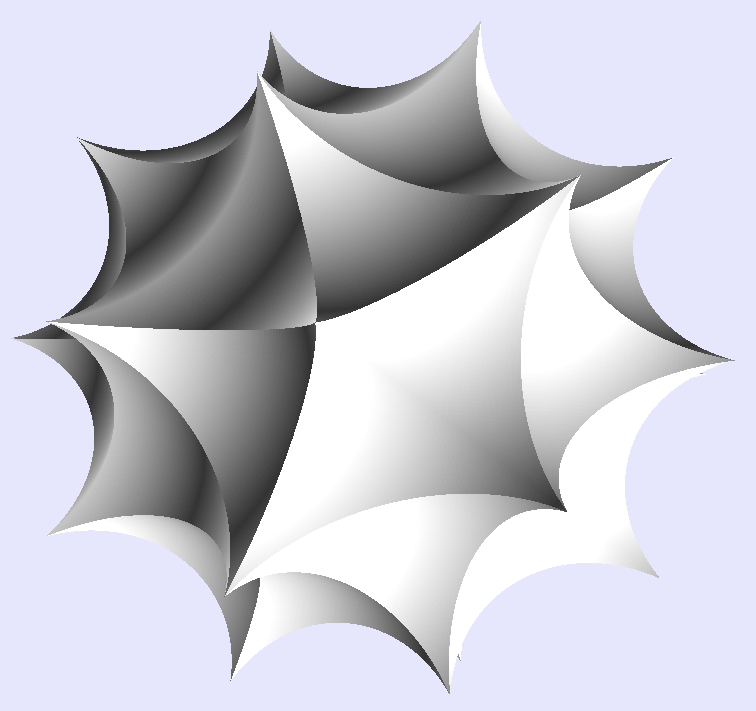
\includegraphics[width=3in]{icosahedron.png}
\end{center}
\end{columns}
}
\frame
{
\begin{columns}[c]
\column{1.1in}
The symmetry group of a 
\textcolor{red}{Euclidean tessellation}
is a Kleinian group
by stereographic
projection.
\column{3in}
\begin{center}
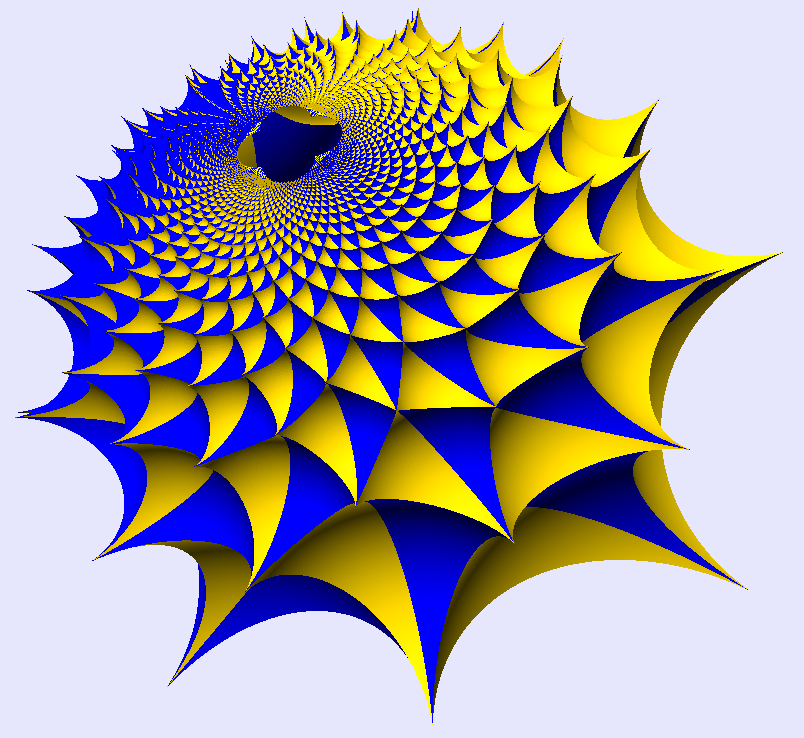
\includegraphics[width=3in]{parabolic.png}
\end{center}
\end{columns}
}
\frame
{
\begin{columns}[c]
\column{1.1in}
A Kleinian group 
preserving a round circle
on the sphere is a
\textcolor{blue}{Fuchsian group}.
\column{3in}
\begin{center}
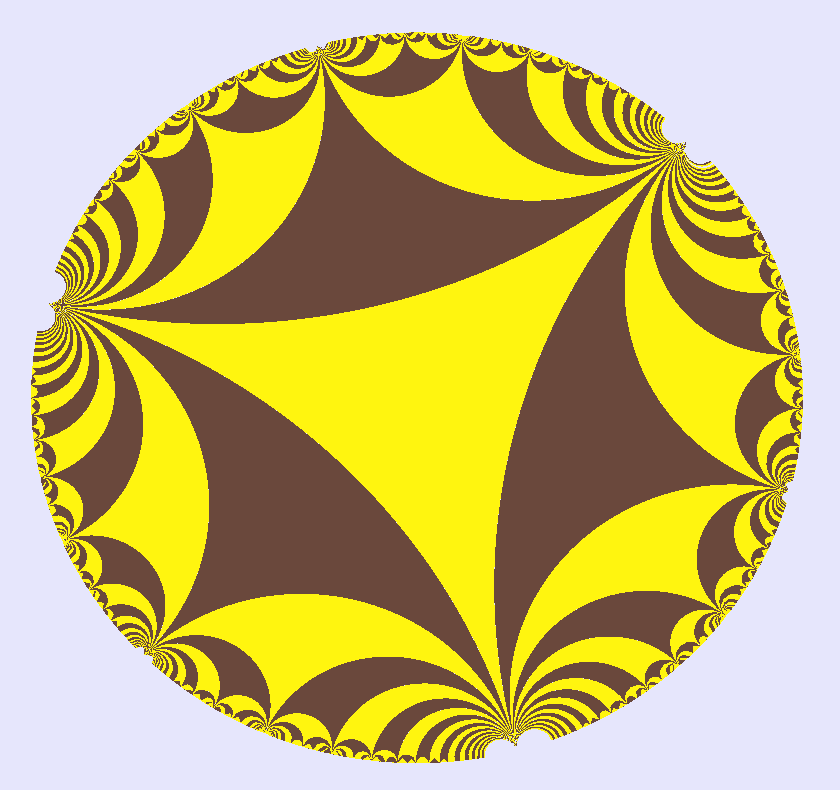
\includegraphics[width=3in]{fuchsian.png}
\end{center}
\end{columns}
}
\frame
{
And there are many other examples.
\begin{center}
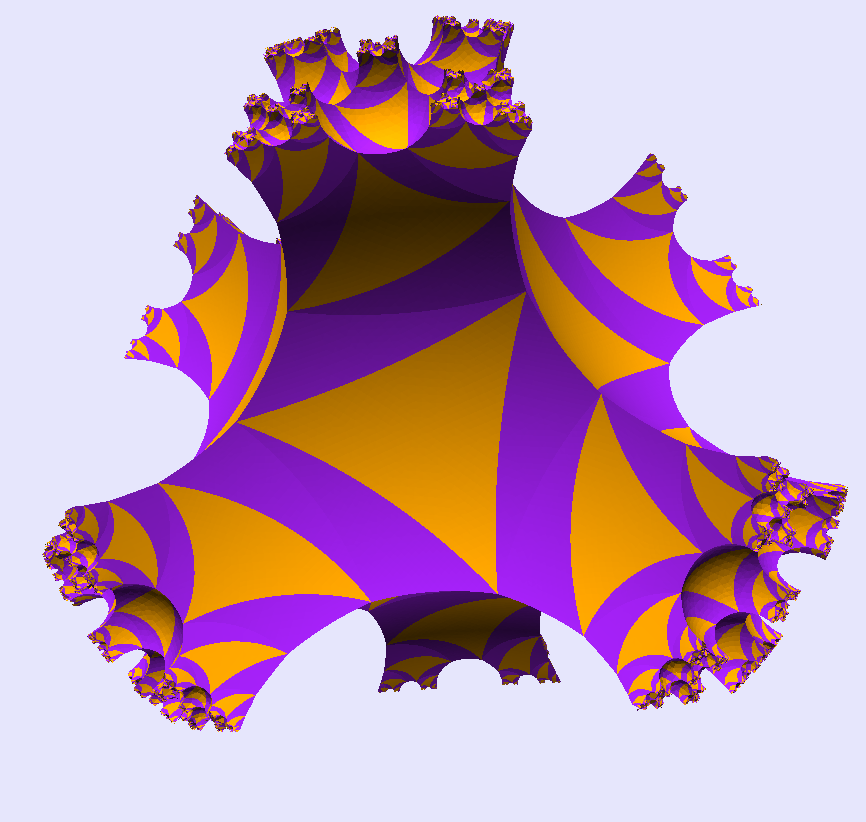
\includegraphics[width=2in]{Schottky.png}\hskip 2pt
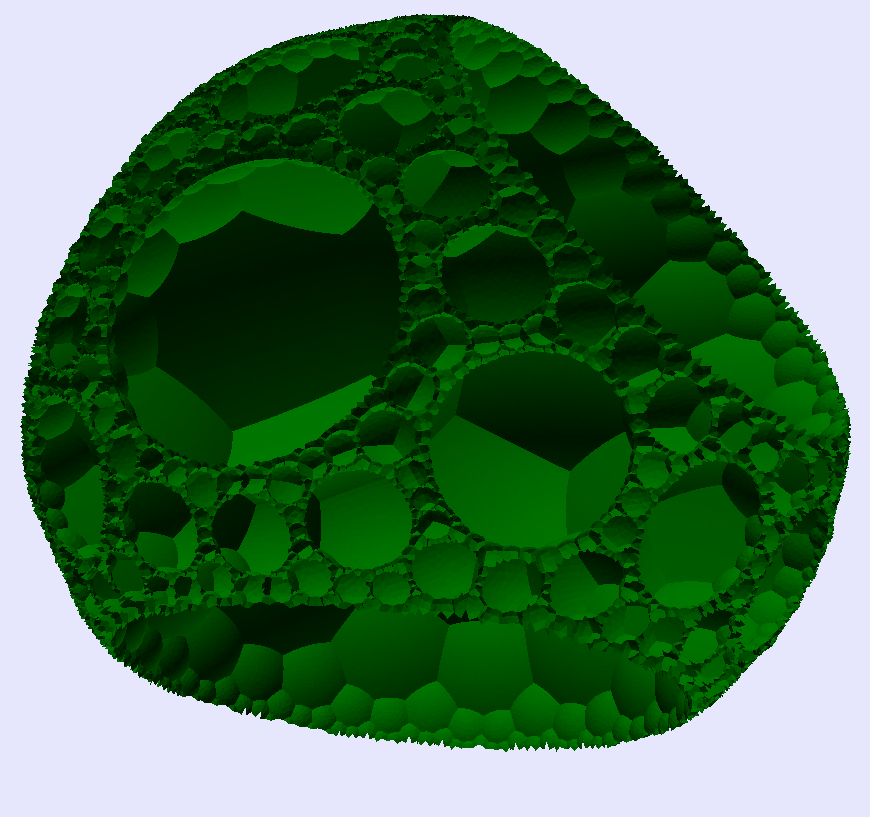
\includegraphics[width=2in]{7gon_spine.png}
\end{center}
}
\frame
{
If we identify the unit sphere with the \textcolor{dgreen}{Riemann sphere} 
$$S^2 = \CP^1:=\C\cup \infty$$
then (orientation-preserving) conformal symmetries are \textcolor{red}{fractional linear
transformations}
$$z \to \frac {az+b} {cz+d}$$
and the group of all such transformations is $\PSL(2,\C)$.
}
\frame
{
\frametitle{2. Differential Equations}

Kleinian groups arise in nature as monodromy groups of \textcolor{dgreen}{differential equations}.
\vskip 5pt
Euler introduced the \textcolor{blue}{hypergeometric equation}
$$z(1-z)\frac {d^2w}{dz^2} + [c - (a+b+1)z]\frac {dw}{dz} - abw = 0$$
where $w$ is a function of the variable $z$, and $a$, $b$, $c$ are real constants.
\vskip 10pt
For Euler, $w$ and $z$ were real; but for us they can be complex numbers.
}
\frame
{The space of solutions to the hypergeometric equation
is a complex vector space $V$ of dimension 2. 
\vskip 10pt
There are \textcolor{dgreen}{regular singular points}
at $0$, $1$ and $\infty$, and solutions may be \textcolor{red}{analytically continued} 
around these points.
\vskip 10pt
If $f$ and $g$ are a basis for $V$, the map $$D:z \to f(z)/g(z)$$ is well-defined
in the \textcolor{dgreen}{upper half plane}
$$\HH:=\lbrace z \in \C \text{ with positive imaginary part} \rbrace$$
}
\frame
{
Schwarz showed that the image $D(\HH)$ is a \textcolor{dgreen}{curvilinear triangle} $T$ in $\C$
whose sides are segments of \textcolor{red}{round circles} or \textcolor{red}{straight lines}
and whose angles are $|1-c|\pi$, $|c-a-b|\pi$ and $|a-b|\pi$.
\vskip 10pt
The corners of $T$ are the images of $0$, $1$ and $\infty$.
\begin{center}
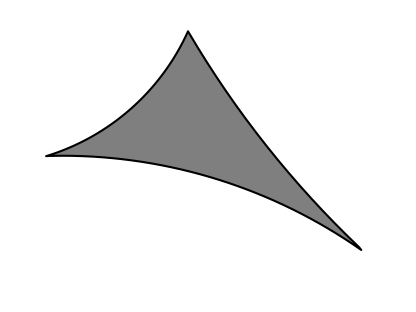
\includegraphics[width=3in]{Schwarz_triangle.png}
\end{center}
}
\frame
{
If we \textcolor{red}{analytically continue} $D$ across a segment of 
$\R - \lbrace 0,1,\infty\rbrace$, it maps
the lower half plane $\overline{\HH}$ onto a triangle obtained from $T$ by \textcolor{dgreen}{inversion}
in the corresponding circular side (or \textcolor{dgreen}{reflection} in a straight side).
\vskip 10pt
Continuing $D$ around loops, we get a
representation 
$$D_*:\pi_1(\CP^1 - \lbrace 0,1,\infty\rbrace) \to \PSL(2,\C)$$ 
}
\frame
{
If the angles of the curvilinear triangle $T$ are of the form $\pi/n$ for integers $n$, 
the image of $D_*$ is discrete, and hence is a Kleinian group
called a \textcolor{blue}{triangle group}.
\begin{center}
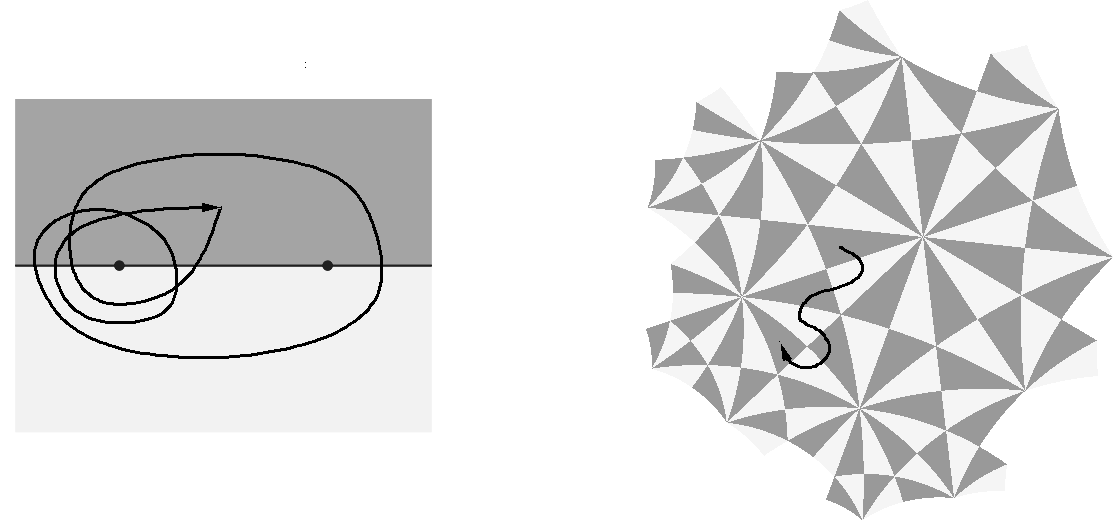
\includegraphics[width=4in]{triangle_group.png}
\end{center}
}
\frame
{
\frametitle{3. Hyperbolic geometry}
Poincar\'e realized that $\PSL(2,\C)$ is also the group
of (orientation-preserving) \textcolor{red}{isometries} of hyperbolic 3-space $\H^3$.
\vskip 10pt
In Poincar\'e's model, $\H^3$ is the interior of the unit ball.
The hyperbolic metric is obtained by rescaling the Euclidean metric
by a factor of $2/(1-r^2)$ where $r$ is the distance to $0$.
\vskip 10pt
Straight lines in the Poincar\'e metric are arcs of Euclidean
straight lines or circles perpendicular to the boundary sphere.
}
\frame
{
\begin{columns}[c]
\column{1.1in}
In the Poincar\'e
metric, objects near the
boundary sphere look
smaller.
\column{3in}
\begin{center}
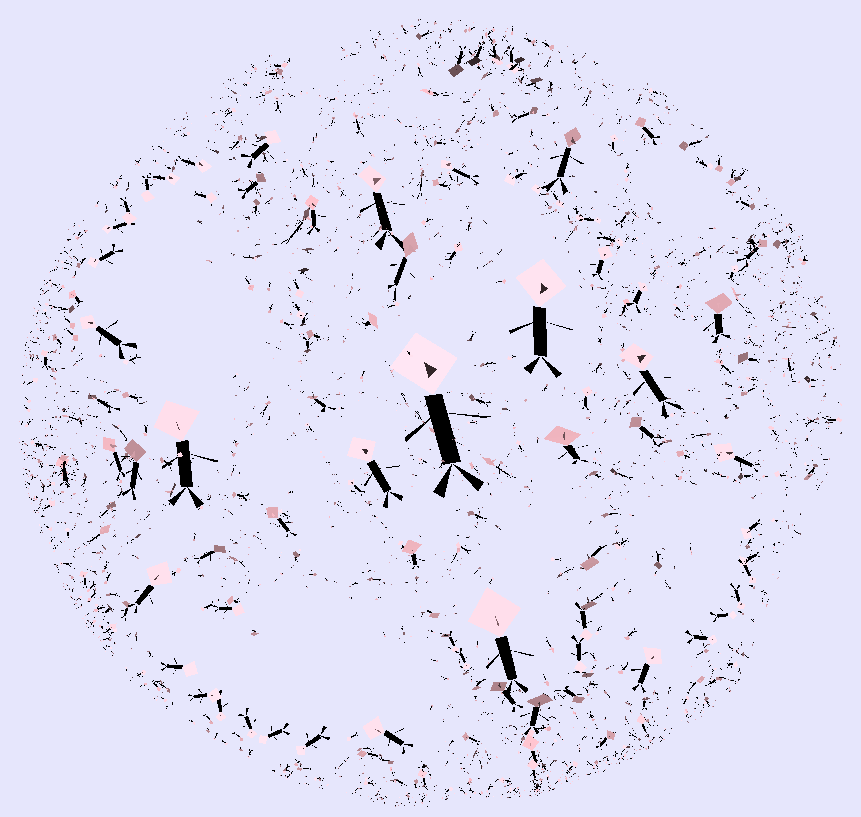
\includegraphics[width=3in]{Poincare.png}
\end{center}
\end{columns}
}
\frame
{
If $\Gamma$ is a torsion-free Kleinian group, then
$\Gamma$ acts \textcolor{red}{freely} and \textcolor{red}{properly discontinuously}
on $\H^3$ by isometries.
\vskip 10pt
Thus the quotient $M:=\H^3/\Gamma$ is a \textcolor{blue}{hyperbolic manifold}
with universal cover $\H^3$, and fundamental group $\pi_1(M)\cong \Gamma$.
\vskip 10pt
Conversely, every 3-manifold $M$ with a \textcolor{red}{complete} hyperbolic
metric has universal cover $\widetilde{M}$ isometric to $\H^3$, realizing
the deck group $\pi_1(M)$ as a Kleinian group $\Gamma$.
}
\frame
{
Thurston conjectured, and Perelman proved, the 
\vskip 10pt
\textcolor{blue}{Geometrization Theorem}: a closed 3-manifold $M$ admits a hyperbolic structure if and only if
\begin{enumerate}
\item{every smooth embedded sphere in $M$ bounds a ball;}
\item{$\pi_1(M)$ is infinite; and}
\item{$\pi_1(M)$ contains no $\Z^2$ subgroup.}
\end{enumerate}
}
\frame
{
\frametitle{4. Dynamics}
If $\Gamma$ is a Kleinian group, the sphere $S^2$ decomposes into 
\begin{enumerate}
\item{the \textcolor{blue}{Limit set} 
$\Lambda$ where $\Gamma$ acts \textcolor{red}{ergodically}, and}
\item{the \textcolor{blue}{Domain of discontinuity}
$\Omega$ where $\Gamma$ acts \textcolor{red}{properly discontinuously}.}
\end{enumerate}
$\Lambda$ is closed, and $\Omega$ is open. For torsion-free 
Kleinian groups, $\Lambda$ is the closure of the set of fixed points of $\Gamma$.
\vskip 10pt
The quotient $\Omega/\Gamma$ is a Riemann surface. Ahlfors showed it is of
\textcolor{dgreen}{finite type}; i.e.\/ it is homeomorphic to a compact surface
minus finitely many points.
}
\frame
{
A random walk in the Euclidean plane is \textcolor{red}{recurrent}. In higher dimensions, it diverges, but
very slowly and chaotically.
\begin{columns}[c]
\column{2in}
\begin{center}
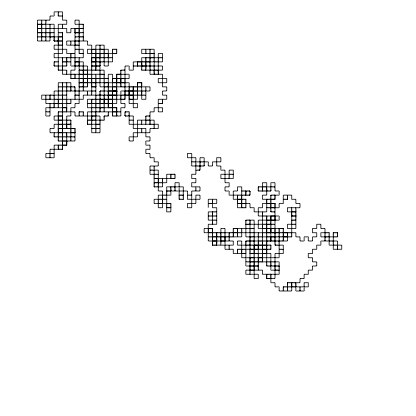
\includegraphics[width=2in]{turtle_Euclid.png}
\end{center}
\column{2in}
\begin{center}
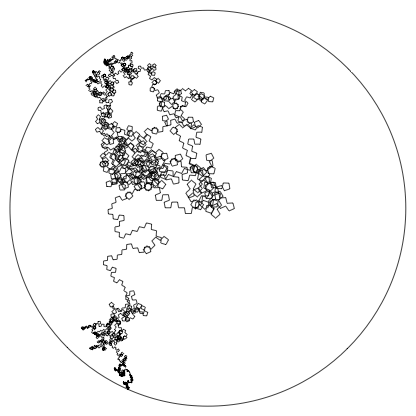
\includegraphics[width=2in]{turtle_hyperbolic.png}
\end{center}
\end{columns}
In hyperbolic space of any dimension, the negative curvature \textcolor{dgreen}{freezes} 
the trajectory of a random walk, so that it converges to a definite point on the sphere
at infinity.
}
\frame
{
If $\Gamma$ is a Kleinian group, \textcolor{red}{measurable functions} on $\Omega/\Gamma$
are the asymptotic values of \textcolor{red}{harmonic functions} on the hyperbolic
manifold $M:=\H^3/\Gamma$.
\vskip 10pt
So whenever $\Lambda$ is not equal to $S^2$ there are many harmonic functions on $M$.
\begin{center}
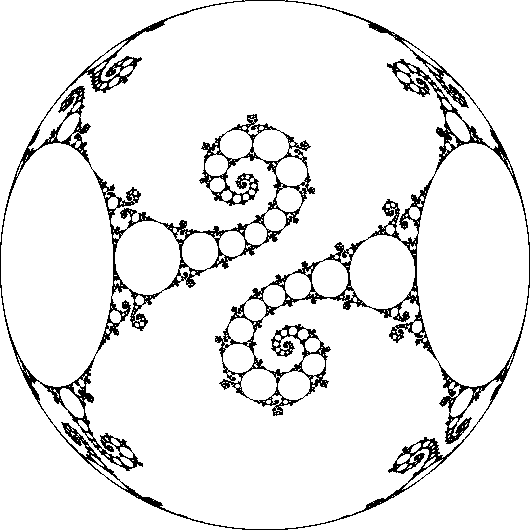
\includegraphics[width=1in]{ctm_cusp.png}\hskip 13pt
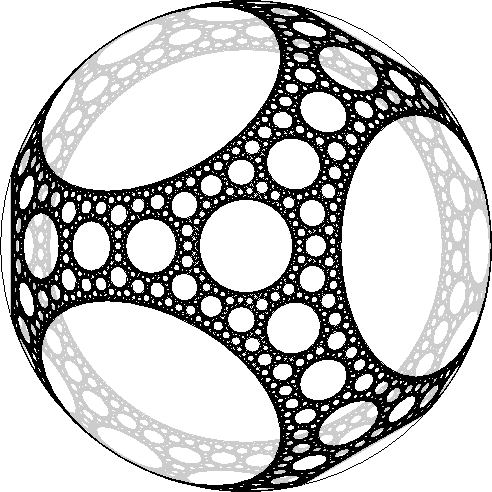
\includegraphics[width=1in]{ctm_carpet.png}\hskip 8pt
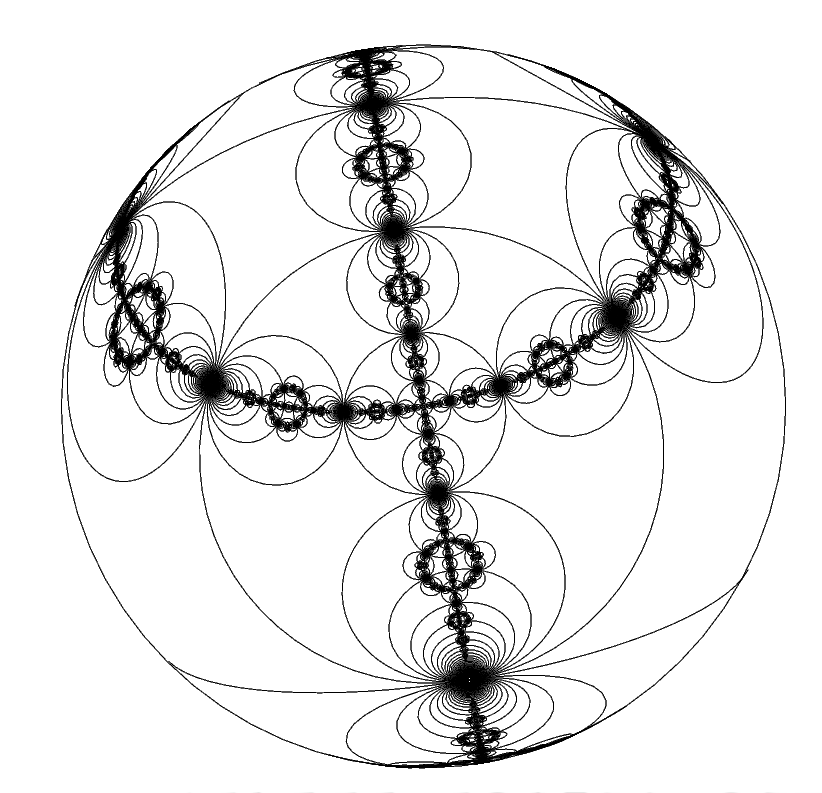
\includegraphics[width=1.1in]{ctm_cylindrical.png}
\end{center}
\begin{center}
\small{limit set images by Curt McMullen}
\end{center}
}
\frame
{
If $M$ is a closed hyperbolic manifold, there are no nonconstant harmonic functions on $M$,
by the \textcolor{dgreen}{maximum principle}. So $\Lambda = S^2$.
\vskip 10pt
But it {\em is} possible for $\Lambda = S^2$ even if $M$ is noncompact!
}
\frame
{
\textcolor{blue}{Example:} $\Sigma$ is a surface, and $\phi:\Sigma \to \Sigma$ is
a diffeomorphism. Define the \textcolor{red}{mapping torus}
$$M_\phi:=\Sigma\times [0,1]/(s,1)\sim(\phi(s),0)$$
which is topologically a bundle over $S^1$ with fiber $\Sigma$:
$$\Sigma \to M_\phi \to S^1$$
}
\frame
{
There is a corresponding short exact sequence of fundamental groups
$$0 \to \pi_1(\Sigma) \to \pi_1(M_\phi) \to \Z \to 0$$
In particular, $\pi_1(\Sigma)$ is a \textcolor{red}{normal} subgroup of $\pi_1(M_\phi)$.
\vskip 10pt
If $\phi$ is sufficiently complicated, Thurston showed $M_\phi$ is hyperbolic.
}
\frame
{
Let $\widehat{M}_\phi$ be the infinite cover of $M_\phi$ with fundamental group
$\pi_1(\Sigma)$. Topologically, $\widehat{M}_\phi = \Sigma \times \R$.
\vskip 10pt
Since $\pi_1(\Sigma)$ is \textcolor{red}{normal} in $\pi_1(M_\phi)$, it follows that
$\Lambda(\widehat{M}_\phi)$ is invariant under all of $\pi_1(M_\phi)$; in fact
$$\Lambda(\widehat{M}_\phi) = \Lambda(M_\phi)$$
But $M_\phi$ is closed, so $\Lambda(M_\phi)=S^2$.
}
\frame
{
Each fiber $\Sigma$ is a surface, whose universal cover
$\widetilde{\Sigma}$ is topologically a plane, which is properly embedded in
$\widetilde{M}_\phi\cong \H^3$.  
\vskip 10pt
This plane accumulates on $\Lambda(\widehat{M}_\phi)=S^2$; i.e.\/ it limits to all
of $S^2$!
\begin{center}
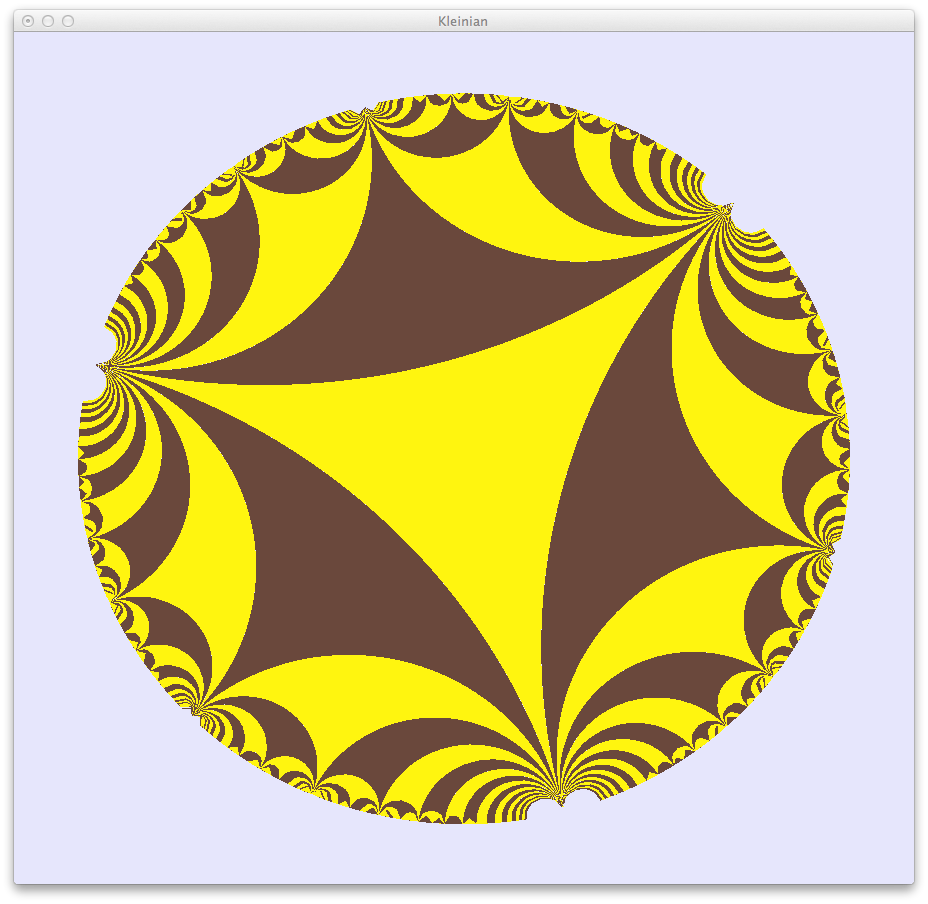
\includegraphics[width=1in]{torus_0.png}\hskip 4pt
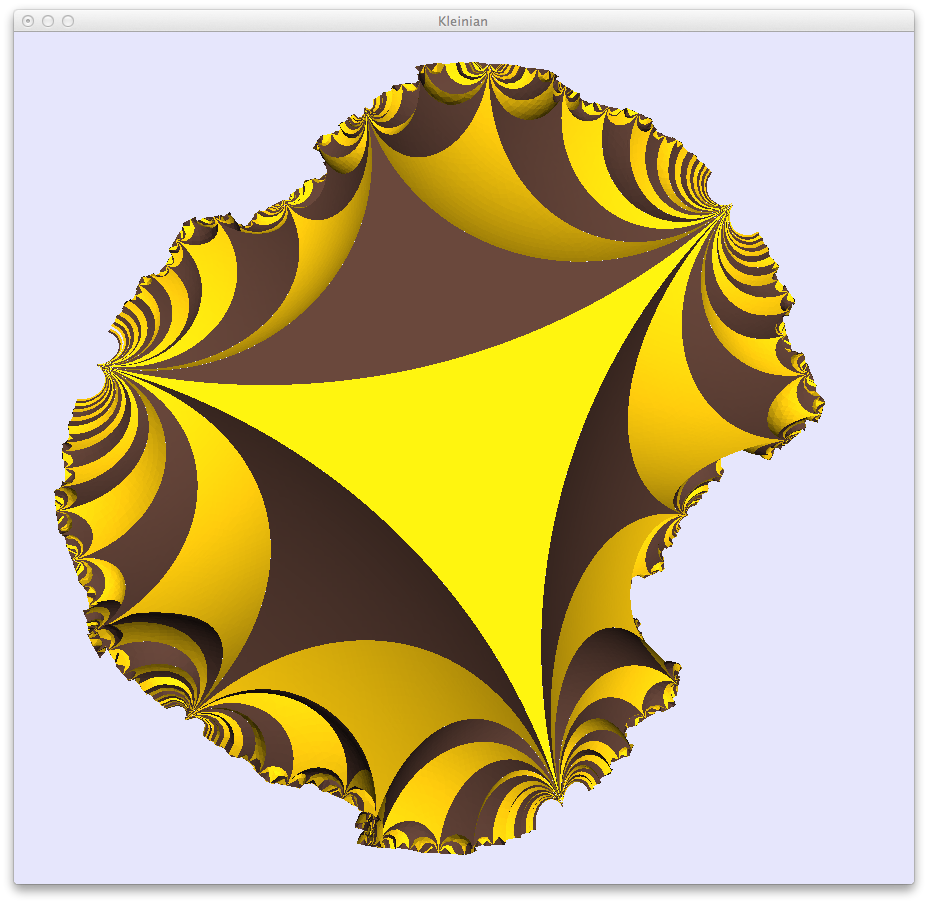
\includegraphics[width=1in]{torus_12.png}\hskip 4pt
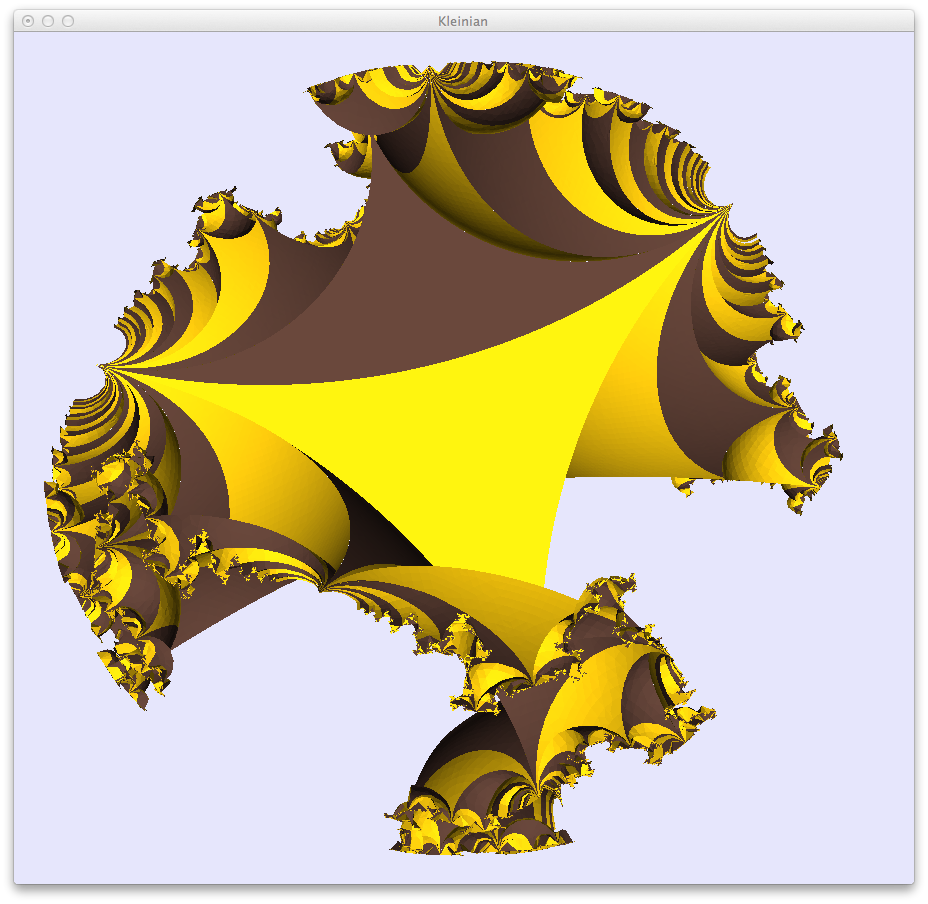
\includegraphics[width=1in]{torus_24.png}\hskip 4pt
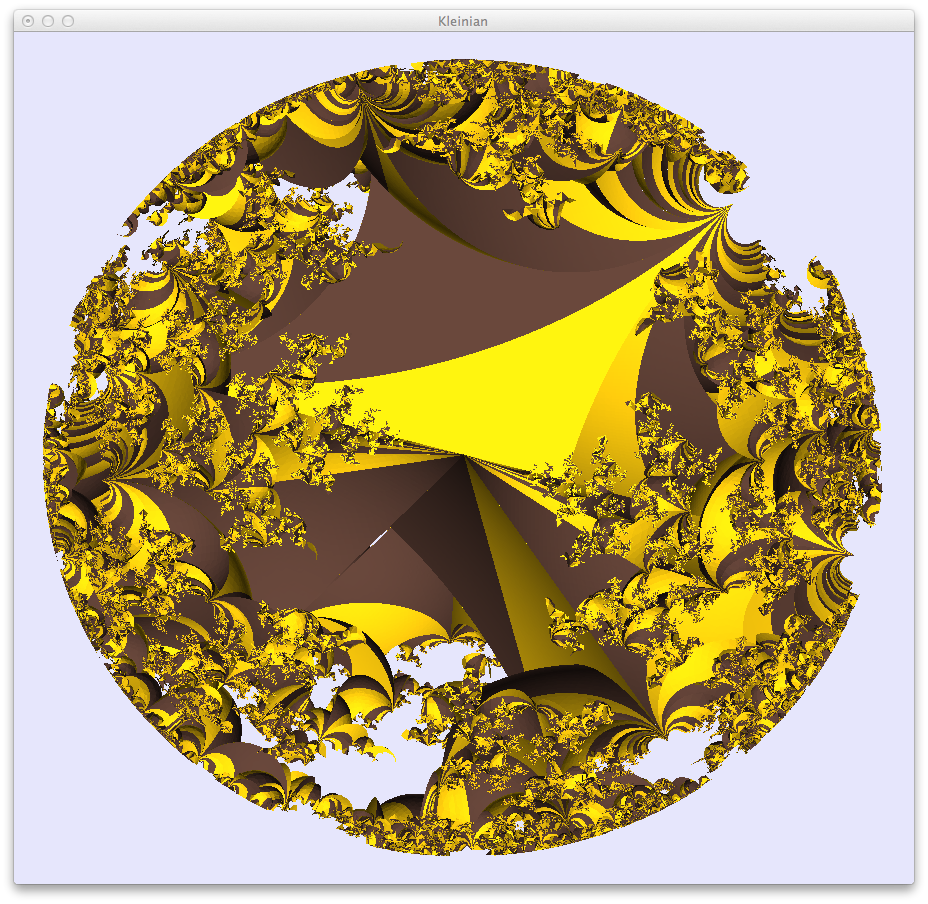
\includegraphics[width=1in]{torus_36.png}
\end{center}
\begin{center}$\langle${\sl show movie}$\rangle$\end{center}
}
\frame
{
\frametitle{5. Ahlfors' Conjecture and Tameness}
In 1966, Ahlfors formulated his
\vskip 10pt
\textcolor{blue}{Ahlfors Measure Conjecture:} If $\Gamma$ is a Kleinian group, then either
$\Lambda=S^2$ or $\Lambda$ has measure zero.
\vskip 10pt
If $\Gamma$ violates Ahlfors conjecture, we can build a function $\chi_\Lambda$ on $S^2$
which is $1$ on $\Lambda$ and $0$ on $\Omega$, and a nonconstant harmonic function
$h_\Lambda$ on $M:=\H^3/\Gamma$ which is zero on $\Omega/\Gamma$.
}
\frame
{
A random walk preserves the value of a harmonic function \textcolor{dgreen}{on average}.
If $\Gamma$ violates Ahlfors conjecture, a random walk on $M:=\H^3/\Gamma$ has
a definite chance of failing to converge to $\Omega/\Gamma$.
\vskip 10pt
Where else can a random walk go? It has to go into one of the \textcolor{dgreen}{ends} of $M$
and \textcolor{red}{stay there}.
}
\frame
{
The manifold $M:=\H^3/\Gamma$ has $\pi_1(M)\cong\Gamma$ which is finitely generated.
\vskip 10pt
The \textcolor{blue}{Scott Core Theorem} says that there is a \textcolor{red}{compact}
\textcolor{blue}{core}
$C \subset M$ such that $C \to M$ is a homotopy equivalence.
\vskip 10pt
The \textcolor{dgreen}{ends} of $M$ are the components of $M-C$.
\vskip 10pt
Some of these ends limit to components of $\Omega/\Gamma$; these are the 
\textcolor{red}{geometrically finite} ends.
}
\frame
{
\textcolor{blue}{Example:} The cyclic cover $\widehat{M}_\phi=\Sigma \times \R$ has two \textcolor{red}{geometrically
infinite} ends. The surfaces $\Sigma \times t$ have bounded area, 
so a random walk on $\widehat{M}_\phi$ looks like a random walk on $\R$.
\vskip 10pt
But a random walk on $\R$ is \textcolor{red}{recurrent}! So the random walk on $\widehat{M}_\phi$ will not
stay in either of the ends, but keep coming back to any compact region.
}
\frame
{
Thurston and Canary showed that to prove Ahlfors Conjecture, it suffices to show that the
ends of $M:=\H^3/\Gamma$ are all topologically products $\Sigma \times \R^+$. Such ends
are said to be \textcolor{dgreen}{tame}.
\vskip 10pt
In 1974, Marden conjectured that all hyperbolic manifolds $M:=\H^3/\Gamma$ are 
\textcolor{dgreen}{tame}; equivalently, they are all homeomorphic to the interior of a
compact 3-manifold, possibly with boundary.
\vskip 10pt
In 2004, Marden's \textcolor{blue}{Tameness Conjecture} was proved independently by
Agol and by Calegari--Gabai; thus by the combined work of many people,
we know that Ahlfors' Conjecture is true.
}
\frame
{
\begin{block}{References}
\begin{itemize}
\item{D. Mumford, C. Series and D. Wright, {\em Indra's Pearls: The Vision of Felix Klein}.}
\item{W. Thurston, {\em Three dimensional manifolds, Kleinian groups and hyperbolic geometry},
Bull. AMS, 1982}
\end{itemize}
\end{block}
}

\end{document}

